\begin{enumerate}[label=\bfseries Câu \arabic*:]

	\item \mkstar{1}

\cauhoi{
	
	Hiện tượng giao thoa là hiện tượng
	
	\begin{mcq}(1)
		\item tổng hợp của hai dao động.
		\item tạo thành các gợn lồi, lõm.
		\item hai sóng kết hợp khi gặp nhau thì có những điểm chúng luôn tăng cường, có những điểm chúng luôn luôn triệt tiêu nhau.
		\item giao nhau của hai sóng tại một điểm của môi trường.
	\end{mcq}
}

\loigiai{
	\textbf{Đáp án C.}
	
		Hiện tượng giao thoa là hiện tượng hai sóng kết hợp khi gặp nhau thì có những điểm chúng luôn tăng cường, có những điểm chúng luôn luôn triệt tiêu nhau.
}
	\item \mkstar{1}

\cauhoi{
	
	Tại hai điểm A, B trên mặt nước nằm ngang có hai nguồn sóng cơ kết hợp, cùng biên độ, ngược pha, dao động theo phương thẳng đứng. Coi biên độ sóng lan truyền trên mặt nước không đổi trong quá trình truyền sóng. Phần tử nước thuộc trung điểm của đoạn AB 
	
	\begin{mcq}
		\item Dao động với biên độ bằng biên độ dao động của mỗi nguồn.
		\item Không dao động.
		\item Dao động có biên độ gấp đôi biên độ của nguồn.
		\item Dao động với biên độ nhỏ hơn biên độ dao động của mồi nguồn.
	\end{mcq}
	
}

\loigiai{
	\textbf{Đáp án B.}
	
	Do 2 nguồn ngược pha nên khi có sự giao thoa hai sóng đó trên mặt nước thì dao động tại trung điểm của đoạn S$_1$S$_2$ có biên độ cực tiểu là 0 (hay không dao động).
}
	\item \mkstar{1}

\cauhoi{
	
	Giao thoa ở mặt nước với hai nguồn sóng kết hợp đặt tại A và B dao động điều hòa cùng pha theo phương thẳng đứng. Sóng truyền ở mặt nước có bước sóng $\lambda$ . Cực tiểu giao thoa nằm tại những điểm có hiệu đường đi của hai sóng từ hai nguồn tới đó bằng
	
	\begin{mcq}(2)
		\item $(k+1)\lambda$ với $k = 0,\pm1,\pm 2,...$.
		\item $k\lambda $ với $k = 0,\pm1,\pm 2,...$.
		\item $(k+ \text{0,5})\lambda $ với $k = 0,\pm1,\pm 2,...$.
		\item $2k\lambda $ với $k = 0,\pm1,\pm 2,...$.
	\end{mcq}
	
}

\loigiai{
	\textbf{Đáp án C.}
	
	Giao thoa ở mặt nước với hai nguồn sóng kết hợp đặt tại A và B dao động điều hòa cùng pha theo phương thẳng đứng. Sóng truyền ở mặt nước có bước sóng $\lambda$ .
	
	Cực tiểu giao thoa nằm tại những điểm có hiệu đường đi của hai sóng từ hai nguồn tới đó bằng  $(k+ \text{0,5})\lambda $ với $k = 0,\pm1,\pm 2,...$
}
	\item \mkstar{1}

\cauhoi{
	
	Ở mặt nước có hai nguồn sóng dao động theo phương vuông góc với mặt nước, có cùng phương trình $u = A\cos\omega t$. Trong miền gặp nhau của hai sóng, những điểm mà ở đó các phần tử nước dao động với biên độ cực đại sẽ có hiệu đường đi của sóng từ hai nguồn đến đó bằng
	
	\begin{mcq}(2)
		\item một số lẻ lần bước sóng.
		\item một số nguyên lần nửa bước sóng.
		\item một số lẻ lần nửa bước sóng.
		\item một số nguyên lần bước sóng.
	\end{mcq}
	
}

\loigiai{
	\textbf{Đáp án D.}
	
	Ở mặt nước có hai nguồn sóng dao động theo phương vuông góc với mặt nước, có cùng phương trình $u = A\cos\omega t$. Trong miền gặp nhau của hai sóng, những điểm mà ở đó các phần tử nước dao động với biên độ cực đại sẽ có hiệu đường đi của sóng từ hai nguồn đến đó bằng một số nguyên lần bước sóng
}
\item \mkstar{2}

\cauhoi{
	
	Cho phương trình sóng: $u=a\sin\left(7\pi t+\dfrac{\pi}{3}+\dfrac{4\pi x}{10}\right)\ \text{(m,s)}$ . Phương trình này biểu diễn: 
	
	\begin{mcq}
		\item Sóng chạy theo chiều âm của trục x với vận tốc $\dfrac{10}{7}\ \text{m/s}$.
		\item Sóng chạy theo chiều âm của trục x với vận tốc $\dfrac{175}{10}\ \text{m/s}$.
		\item Sóng chạy theo chiều dương của trục x với vận tốc $\dfrac{175}{10}\ \text{m/s}$.
		\item Sóng chạy theo chiều dương của trục x với vận tốc $\dfrac{10}{7}\ \text{m/s}$.
	\end{mcq}
	
}

\loigiai{
	\textbf{Đáp án C.}
	
	Giả sử phương trình sóng tổng quát có dạng: 
	
	$u=A \cos\left(\omega t+\varphi +2\pi \dfrac{x}{\lambda}\right)$. 
	
	Theo phương trình sóng tổng quát ta có: $\omega = 7\pi\ \text{rad/s} \Rightarrow$ $T=\dfrac{2}{7}\ \text{s}$. 
	
	$\dfrac{2\pi}{\lambda}=\text{0,4}\pi\Rightarrow \lambda = \SI{5}{m}$. 
	
	$v=\dfrac{\lambda}{T}=\dfrac{175}{10}\ \text{cm/s}$. 
	
	Vì $\Delta\varphi=+\dfrac{4\pi x}{10}$ nên sóng chạy theo chiều dương của trục x với vận tốc $\dfrac{175}{10}\ \text{m/s}$.
}
\item \mkstar{2}

\cauhoi{
	
	Trong thí nghiệm giao thoa sóng ở mặt nước, hai nguồn kết hợp đặt tại hai điểm A và B dao động cùng pha theo phương thẳng đứng. Trên đoạn thẳng AB, khoảng cách giữa hai cực đại giao thoa liên tiếp là 2 cm. Sóng truyền trên mặt nước có bước sóng là
	
	\begin{mcq}(4)
		\item 8 cm.
		\item 2 cm.
		\item 4 cm.
		\item 1 cm.
	\end{mcq}
	
}

\loigiai{
	\textbf{Đáp án C.}
	
	Khoảng cách giữa hai cực đại giao thoa liên tiếp bằng $\dfrac{\lambda}{2}$. Nên bước sóng là $\SI{4}{cm}$.
}
\item \mkstar{2}

\cauhoi{
	
	Để khảo sát giao thoa sóng cơ, người ta bố trí trên mặt nước nằm ngang hai nguồn kết hợp S$_1$ và S$_2$. Hai nguồn này dao động điều hòa theo phương thẳng đứng, cùng pha. Xem biên độ sóng không thay đổi trong quá trình truyền sóng. Các điểm thuộc mặt nước và nằm trên đường trung trực của đoạn S$_1$S$_2$ sẽ
	
	\begin{mcq}
		\item dao động với biên độ bằng nửa biên độ cực đại.
		\item dao động với biên độ cực đại.
		\item dao động với biên độ cực tiểu.
		\item không dao động.
	\end{mcq}
	
}

\loigiai{
	\textbf{Đáp án B.}
	
	Các điểm thuộc mặt nước và nằm trên đường trung trực của đoạn S$_1$S$_2$ có hiệu đường đi bằng 0 nên sẽ dao động với biên độ cực đại.
}
	\item \mkstar{2}

\cauhoi{
	
	Thực hiện thí nghiệm giao thoa sóng cơ trên mặt nước với hai nguồn cùng pha có tần số 10 Hz, vận tốc truyền sóng trên mặt nước là 50 cm/s. Hỏi tại vị trí M cách nguồn 1 một đoạn $d_1=\SI{20}{cm}$ và cách nguồn 2 một đoạn $d_2 = \SI{25}{cm}$, là điểm cực đại hay cực tiểu, và là cực đại hay cực tiểu số mấy?	
	\begin{mcq}(2)
		\item Cực tiểu số 1.
		\item Cực đại số 1.
		\item Cực đại số 2.
		\item Cực tiểu số 2.
	\end{mcq}
	
}

\loigiai{
	\textbf{Đáp án B.}
	
	Ta có $d_2-d_1=\SI{5}{cm}$ và $\lambda = \dfrac{v}{f} =\SI{5}{cm}$. 
	
	
	Vì $\Delta d =\lambda \Rightarrow k=1$.
	
	Vậy điểm M nằm trên đường cực đại số 1.
}

\item \mkstar{2}

\cauhoi{
	
	Thực hiện thí nghiệm giao thoa sóng cơ trên mặt nước với hai nguồn cùng pha có tần số 10 Hz, vận tốc truyền sóng trên mặt nước là 50 cm/s. Hỏi tại vị trí M cách nguồn 1 một đoạn $d_1=\SI{17,5}{cm}$ và cách nguồn 2 một đoạn $d_2 = \SI{25}{cm}$, là điểm cực đại hay cực tiểu, cực đại hay cực tiểu số mấy?	
	\begin{mcq}(2)
		\item Cực tiểu số 1.
		\item Cực đại số 1.
		\item Cực đại số 2.
		\item Cực tiểu số 2.
	\end{mcq}
	
}

\loigiai{
	\textbf{Đáp án D.}
	
	Ta có $d_2-d_1=\SI{7,5}{cm}$ và $\lambda = \dfrac{v}{f} =\SI{5}{cm}$. 
	
	
	Vì $\Delta d =\text{1,5}$.
	
	Vậy điểm M nằm trên đường cực tiểu số 2.
}
	\item \mkstar{2} 

\cauhoi{
	
	Trong thí nghiệm giao thoa sóng trên mặt nước hai nguồn kết hợp A, B cách nhau 12,5 cm dao động cùng pha với tần số 10 Hz. Tốc độ truyền sóng trên mặt nước là 20 cm/s. Số đường dao động cực đại trên mặt nước là	
	\begin{mcq}(2)
		\item 13 đường.
		\item 11 đường.
		\item 15 đường.
		\item 12 đường.
	\end{mcq}
	
}

\loigiai{
	\textbf{Đáp án A.}
	
	Hai nguồn cùng pha ($\Delta \varphi =0$).
	
	Cực đại: $-\dfrac{L}{\lambda} \leq k \leq \dfrac{L}{\lambda}$. 
	
	$\Rightarrow -\text{6,25} \leq k \leq \text{6,25}$.
	
	Có 13 giá trị của $k$.
	
}
	\item \mkstar{2}

\cauhoi{
	
	Tại hai điểm O$_1$O$_2$ cách nhau 48 cm trên mặt chất lỏng có 2 nguồn phát sóng dao động theo phương thẳng đứng với phương trình $u_1 = 5\cos 100\pi t\ \text{mm}$; $u_2 = 5\cos \left(100\pi t + \dfrac{\pi}{2}\right)\ \text{mm}$. Vận tốc truyền sóng trên mặt thoáng chất lỏng là 2 m/s. Coi biên độ sóng không đổi trong quá trình truyền sóng. Số điểm trên đoạn O$_1$O$_2$ dao động với biên độ cực đại (không kể O$_1$, O$_2$) là	
	\begin{mcq}(4)
		\item 23.
		\item 24.
		\item 25.
		\item 26.
	\end{mcq}
	
}

\loigiai{
	\textbf{Đáp án B.}
	
	Hai nguồn dao động vuông pha: $\Delta \varphi =\dfrac{\pi}{2}$. 
	
	Số cực đại: $-\dfrac{L}{\lambda}-\dfrac{\Delta \varphi}{2\pi} \leq k \leq \dfrac{L}{\lambda}-\dfrac{\Delta \varphi}{2\pi} \Rightarrow -\text{12,5} \leq k \leq \text{11,75}$.
	
	Có 24 điểm.
}
\item \mkstar{2}

\cauhoi{
	
	Thực hiện thí nghiệm giao thoa sóng cơ trên mặt nước với hai nguồn cùng pha có tần số là 10 Hz. M là một điểm cực đại có khoảng cách đến nguồn 1 là $d_1=\SI{25}{cm}$ và cách nguồn 2 là $d_2 = \SI{35}{cm}$. Biết giữa M và đường trung trực còn có 1 cực đại nữa. Xác định bước sóng của sóng trên mặt nước.
	
	\begin{mcq}(4)
		\item 50 cm.
		\item 5 cm.
		\item 50 m.
		\item 5 m.
	\end{mcq}
	
}

\loigiai{
	\textbf{Đáp án B.}
	
	Vì giữa M và đường trung trực còn 1 đường cực đại nữa, nên M nằm trên đường cực đại thứ 2 suy ra $k=2$. 
	
	Ta có: $\Delta d_\text{M} = d_2-d_1 =2\lambda.$
	
	Bước sóng $\lambda =\SI{5}{cm}$.
}
	\item \mkstar{3}	
	
	\cauhoi{		
		Ở mặt nước có hai nguồn sóng cơ A và B cách nhau $15\,\text{cm}$, dao động điều hòa cùng tần số, cùng pha theo phương vuông góc với mặt nước. Điểm M nằm trên AB, cách trung điểm O là $\text{1,5}\,\text{cm}$, là điểm gần O nhất luôn dao động với biên độ cực đại. Trên đường tròn tâm O, đường kính $20\,\text{cm}$, nằm ở mặt nước có số điểm luôn dao động với biên độ cực đại là
		
		\begin{mcq}(4)
			\item 18.
			\item 16.
			\item 32.
			\item 17.
		\end{mcq}		
	}
	
	\loigiai{
		\textbf{Đáp án A.}
		
		\begin{center}
			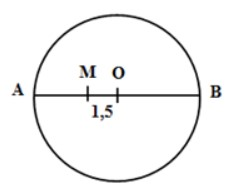
\includegraphics[scale=1.0]{../figs/giaothoasong-h1.jpg}
		\end{center}
		
		Sóng tại M có biên độ cực đại khi $d_2-d_1=k\lambda$.
		
		Ta có $d_1=\dfrac{15}{2}+\text{1,5}=9\,\text{cm}$; $d_2=\dfrac{15}{2}-\text{1,5}=6\,\text{cm}$.
		
		Khi đó $d_2-d_1=3\,\text{cm}$.
		
		Với điểm M gần O nhất, chọn $k=1$.
		
		Khi đó ta có: $\lambda=3\,\text{cm}$.
		
		Số điểm dao động với biên độ cực đại trên đoạn AB là	
		$$-\text{AB}< \text{d}_2-\text{d}_1<\text{AB}$$
		
		Hay $$-15 < k\lambda < 15 \Rightarrow -5 < k < 5$$
		
		Do đó có 9 giá trị $k$.
		
		Do đường kính của đường tròng tâm O là $\text{20}\,\text{cm}$ hai nguồn nằm trong đường tròn nên số điểm dao động với biên độ cực đại trên đường tròn là 18 điểm.
		
	}
	
	%%%%%%%%%%%Câu 2%%%%%%%%%%%%%%
	\item \mkstar{3}
	
	\cauhoi{	
		Hai nguồn sóng kết hợp giống hệt nhau được đặt cách nhau một khoảng cách $x$ trên đường kính của một vòng tròn bán kính $R$ ($x<R$) và đối xứng qua tâm của vòng tròn. Biết rằng mỗi nguồn đều phát sóng có bước sóng $\lambda$ và $x=6\lambda$. Số điểm dao động cực đại trên vòng tròn là
		
		\begin{mcq}(4)
			\item 26.
			\item 24.
			\item 22.
			\item 20.
		\end{mcq}
		
	}
	
	\loigiai{
		\textbf{Đáp án C.}
		
		\begin{center}
			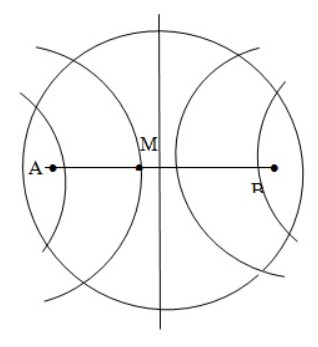
\includegraphics[scale=0.8]{../figs/giaothoasong-h2.jpg}
		\end{center}
		
		Xét điểm M trên AB ($\text{AB}=2x=12\lambda$): $\text{AM}=d_1$ và $\text{BM}=d_2$.
		
		Ta có: $d_1-d_2=k\lambda$ và $d_1+d_2=6\lambda$ nên $d_1=(3+0,5k)\lambda$.
		
		Mặt khác: $0\leq d_1\leq 6\lambda$ nên $-6\leq k \leq 6$.
		
		Số điểm dao động cực đại trên AB  là 13 điểm kể cả hai nguồn A, B, nhưng số đường cực đại cắt đường tròn chỉ có 11. Do đó, số điểm dao động cực đại trên vòng tròn là 22.
		
	}
	
	%%%%%%%%%%%Câu 3%%%%%%%%%%%%%%
	\item \mkstar{3}
	
	\cauhoi{
		
		Trên bề mặt chất lỏng có hai nguồn kết hợp AB cách nhau $40\,\text{cm}$ dao động cùng pha. Biết sóng do mỗi nguồn phát ra có tần số $f=10\,\text{Hz}$, vận tốc truyền sóng $2\,\text{m}/\text{s}$. Gọi M là một điểm  nằm trên đường vuông góc với AB tại đó A dao đông với biên độ cực đại. Đoạn AM có giá trị lớn nhất là
		
		
		\begin{mcq}(4)
			\item $20\,\text{cm}$.
			\item $30\,\text{cm}$.
			\item $40\,\text{cm}$.
			\item $50\,\text{cm}$.
		\end{mcq}
		
	}
	
	\loigiai{
		\textbf{Đáp án B.}
		
		\begin{center}
			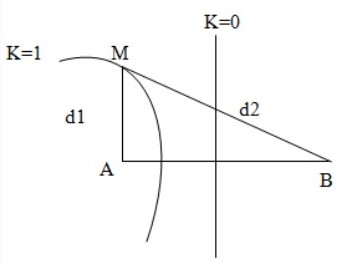
\includegraphics[scale=0.8]{../figs/giaothoasong-h3.jpg}
		\end{center}
		
		Ta có $\lambda = \dfrac{v}{f} = 20\,\text{cm}$.
		
		Do M là một cực đại giao thoa nên để  đoạn AM có giá trị lớn nhất thì M phải nằm trên vân cực đại bậc 1 như hình vẽ và thõa mãn
		$$d_2-d_1=k\lambda=20\,\text{cm}.$$
		
		Mặt khác, do tam giác AMB là tam giác vuông tại A nên ta có
		$$\text{BM}=d_2=\sqrt{\text{AB}^2+\text{AM}^2}=\sqrt{40^2+d_1^2}$$
		
		Từ đó ta suy ra được $d_1=30\,\text{cm}$.
	}
	
	%%%%%%%%%%%Câu 4%%%%%%%%%%%%%%
	\item \mkstar{3} 
	
	\cauhoi{	
		Trên mặt chất lỏng có hai nguồn sóng cùng tần số, cùng pha đặt tại hai điểm A và B. Cho bước sóng do các nguồn gây ra là $\lambda=5\,\text{cm}$. Trên nửa đường thẳng đi qua B trên mặt chất lỏng, hai điểm M và N (N gần B hơn), điểm M dao động với biên độ cực đại, N dao động với biên độ cực tiểu, giữa M và N có ba điểm dao động với biên độ cực đại khác. Biết hiệu $\text{MA}-\text{NA}=\text{1,2}\,\text{cm}$. Nếu đặt hai nguồn sóng này tại M và N thì số điểm dao động với biên độ cực đại trên đoạn thẳng AB là	
		\begin{mcq}(4)
			\item 3.
			\item 4.
			\item 1.
			\item 2.
		\end{mcq}
		
	}
	
	\loigiai{
		\textbf{Đáp án A.}
		\begin{center}
			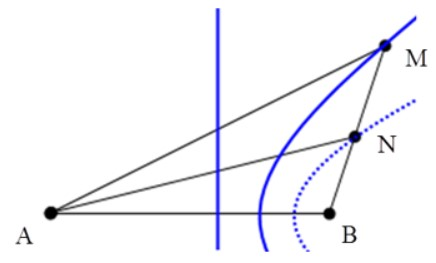
\includegraphics[scale=0.8]{../figs/giaothoasong-h4.jpg}
		\end{center}
		
		M thuộc cực đại và N thuộc cực tiểu nên ta có
		$$\begin{cases}
			\text{AM}-\text{BM}=k\lambda\\
			\text{AN}-\text{BN}=\left[(k+3)+\dfrac{1}{2}\right]\lambda
		\end{cases}
		\Rightarrow\text{MN}=\text{18,7}\,\text{cm}.$$
		
		Với nguồn đặt tại M, N. Xét đoạn AB, ta có
		$$\text{MA}-\text{NA}\leq k\lambda \leq \text{MA}-\text{NB}$$
		$$\Rightarrow \text{0,24}\leq k\lambda \leq\text{3,74}.$$
		
		Vậy có 3 cực đại.
	}
	
	%%%%%%%%%%%Câu 5%%%%%%%%%%%%%%
	\item \mkstar{3}
	
	\cauhoi{
		Ở mặt thoáng của chất lỏng có hai nguồn sóng A, B cách nhau $18\,\text{cm}$, dao động theo phương thẳng đứng với phương trình $u_{\text A}=u_{\text B}=a\cos(20\pi t)$ ($t$ tính bằng s). Tốc độ truyền sóng trên mặt chất lỏng là $50\,\text{cm/s}$. Gọi M là điểm ở mặt chất lỏng gần A nhất sao cho phần tử chất lỏng tại M dao động với biên độ cực đại và cùng pha với nguồn A. Khoảng cách AM là
		\begin{mcq}(4)
			\item $\text{2,5}\,\text{cm}$.
			\item $2\,\text{cm}$.
			\item $5\,\text{cm}$.
			\item $\text{1,25}\,\text{cm}$.
		\end{mcq}
		
	}
	
	\loigiai{
		\textbf{Đáp án C.}
		
		Bước sóng là
		$$\lambda=\dfrac{v}{f}=5\,\text{cm}.$$
		Áp dụng kết quả bài toán điều kiện để một vị trí cực đại và cùng pha với nguồn
		$$\begin{cases}
			d_2-d_1=2k\lambda\\
			d_2+d_1=2m\lambda
		\end{cases}
		\textrm{  hoặc  }
		\begin{cases}
			d_2-d_1=(2k+1)\lambda\\
			d_2+d_1=(2m+1)\lambda
		\end{cases}
		\Rightarrow d_1=(m-k)\lambda.$$
		Do đó $d_{1\ \text{min}}$ khi
		$(m-k)_\text{min}\Rightarrow d_{1\ \text{min}}=\lambda=5\,\text{cm}.$
	}
	
	%%%%%%%%%%%Câu 6%%%%%%%%%%%%%%
	\item \mkstar{3}
	
	\cauhoi{	
		Tại hai điểm A, B trên mặt nước cách nhau $16\,\text{cm}$ có hai nguồn phát sóng giống nhau. Điểm M nằm trên mặt nước và trên đường trung trực của AB cách trung điểm I của AB một khoảng nhỏ nhất bằng $5\sqrt{5}\,\text{cm}$ luôn dao động cùng pha với I. Điểm N nằm trên mặt nước và nằm trên đường thẳng vuông góc với AB tại A, cách A một khoảng nhỏ nhất bằng bao nhiêu để N dao động với biên độ cực tiểu?
		\begin{mcq}(4)
			\item $\text{9,22}\,\text{cm}$.
			\item $\text{8,75}\,\text{cm}$.
			\item $\text{2,14}\,\text{cm}$.
			\item $\text{8,57}\,\text{cm}$.
		\end{mcq}
		
	}
	
	\loigiai{
		\textbf{Đáp án C.}
		
		\begin{center}
			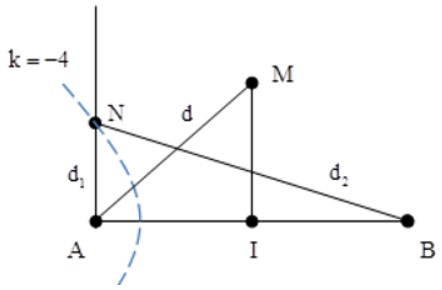
\includegraphics[scale=0.8]{../figs/giaothoasong-h5.jpg}
		\end{center}
		
		Vì hai nguồn đồng pha, M, I đều thuộc trung trực của AB nên để M và I dao động cùng pha thì
		$$\text{MA}-\text{IA}=k\lambda.$$
		M gần I nhất nên $k=1$, do đó
		$$\text{MA}=d_\text{A}=\text{0,5AB}+\lambda=8+\lambda.$$
		Mặt khác $\text{MI}=4\sqrt{5}\,\text{cm}$ nên
		$$\text{MA}=4\sqrt{5}\,\text{cm}\Rightarrow\text{MA}=8+\lambda=\sqrt{\left(\dfrac{\text{AB}}{2}\right)^2+\text{IM}^2}=12\Rightarrow\lambda=4\,\text{cm}.$$
		Số điểm dao động với biên độ cực tiểu trên AB
		$$-\dfrac{\text{AB}}{2}-\dfrac{1}{2}<k<\dfrac{\text{AB}}{2}-\dfrac{1}{2}\Rightarrow-\text{4,5}<k<\text{3,5}.$$
		Để N là một điểm cực tiểu và gần A nhất thì N phải nằm trên hypebol cực tiểu có $k=-4$
		$$\begin{cases}
			d_\text{1N}-d_\text{2N}=-3,5\lambda\\
			d^2_\text{2N}=d^2_\text{1N}+\text{AB}^2
		\end{cases}
		\Rightarrow d_\text{1N}=\text{2,14}\,\text{cm}.$$
	}
	
	%%%%%%%%%%%Câu 7%%%%%%%%%%%%%%
	\item \mkstar{3}
	
	\cauhoi{
		
		Ở mặt nước có hai nguồn kết hợp đặt tại hai điểm A và B, dao động cùng pha theo phương thẳng đứng, phát ra hai sóng có bước sóng $\lambda$. Trên AB có 9 vị trí mà ở đó các phần tử nước dao động với biên độ cực đại. C và D là hai điểm ở mặt nước sao cho ABCD là hình vuông. M là một điểm thuộc cạnh CD và nằm trên vân cực đại giao thoa bậc nhất $\left( \text{MA} -\text{MB}=\lambda\right) $. Biết phần tử tại M dao động cùng pha với các nguồn. Độ dài đoạn AB \textbf{gần nhất} với giá trị nào sau đây?
		
		\begin{mcq}(4)
			\item  $\text{4,6}\lambda$.
			\item $\text{4,8}\lambda$.
			\item $\text{4,4}\lambda$.
			\item $\text{4,7}\lambda$.
		\end{mcq}
		
	}
	
	\loigiai{
		\textbf{Đáp án B.}
		
		\begin{center}
			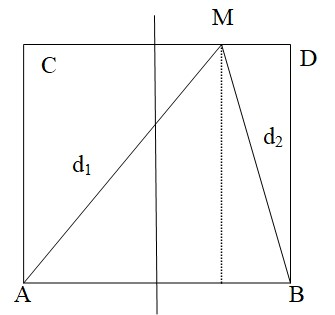
\includegraphics[scale=0.8]{../figs/giaothoasong-h6.jpg}
		\end{center}
		M là cực đại giao thoa và cùng pha với hai nguồn  nên $d_1-d_2=n\lambda, \ d_1+d_2=m\lambda$, với $n, \ m$ là số nguyên cùng lẻ hoặc cùng chẵn.
		
		Vì $n=1\Rightarrow m$ là số lẻ. 
		
		Ta có: $d_1+d_2>\text{AB}, \ 4\lambda \leq \text{AB} < 5\lambda$.
		
		Từ các phương trình trên, ta có: $d_1-d_2=\lambda, \ d_1+d_2=11\lambda$.
		
		Suy ra: $d_1=6\lambda, d_2=5\lambda$.
		
		Ta có:	$\sqrt{(6\lambda)^2-\text{AB}^2}+\sqrt{(5\lambda)^2-\text{AB}^2}=\text{AB}^2\Rightarrow \text{AB}=\text{4,8336}\lambda$.
	}
	%%%%%%%%%%%Câu 8%%%%%%%%%%%%%%
	\item \mkstar{3}
	
	\cauhoi{
		Ở mặt nước, tại hai điểm A và B có hai nguồn kết hợp dao động cùng pha theo phương thẳng đứng. ABCD là hình vuông nằm ngang. Biết trên CD có 3 vị trí mà ở đó các phần tử dao động với biên độ cực đại. Trên AB có tối đa bao nhiêu vị trí mà phần tử ở đó dao động với biên độ cực đại?
		\begin{mcq}(4)
			\item $13$.
			\item $7$.
			\item $11$.
			\item $9$.
		\end{mcq}
		
	}
	
	\loigiai{
		\textbf{Đáp án D.}
		
		Số cực đại trên CD là $a-a\sqrt{2}\leq k\leq a\sqrt{2}-a $.
		
		Chỉ có 3 cực đại $\Rightarrow k=2\Rightarrow \dfrac{a\left(\sqrt{2}-1 \right) }{\lambda}<2\Rightarrow \dfrac{a}{\lambda}<\text{4,8}$.
		
		Số cực đại trên AB là $-a\leq k\leq a\Leftrightarrow -\text{4,8}\leq k\leq \text{4,8}\leq \Rightarrow k=-4; -3,..;3,4$.
		
		Vậy số cực đại trên AB là $9$.
	}
	
	%%%%%%%%%%%Câu 9%%%%%%%%%%%%%%


	\item \mkstar{3}
	
	\cauhoi{
		
		Thực hiện thí nghiệm giao thoa sóng cơ trên mặt chất lỏng với 2 nguồn cùng pha có tần số $f=\SI{30}{Hz}$, vận tốc truyền sóng trong môi trường là 150 cm/s. Trên mặt chất lỏng có 4 điểm có tọa độ so với các nguồn lần lượt như sau: M ($d_1 =\SI{25}{cm}; d_2 = \SI{30}{cm}$); N ($d_1 =\SI{5}{cm}; d_2 = \SI{10}{cm}$); O ($d_1 =\SI{7}{cm}; d_2 = \SI{12}{cm}$); P ($d_1 =\SI{27,5}{cm}; d_2 = \SI{30}{cm}$). Hỏi có mấy điểm nằm trên đường cực đại số 1?	
		
		\begin{mcq}(4)
			\item 1.
			\item 2.
			\item 3.
			\item 4.
		\end{mcq}
		
	}
	
	\loigiai{
		\textbf{Đáp án C.}
		
		
		Ta có $\lambda = \dfrac{v}{f} = \SI{5}{cm}$. 
		
		Tại M: $\Delta d = d_2-d_1 =\SI{5}{cm} =\lambda \Rightarrow$ nằm trên đường cực đại số 1.
		
		Tại N: $\Delta d = d_2-d_1 =\SI{5}{cm} =\lambda \Rightarrow$ nằm trên đường cực đại số 1.
		
		Tại O: $\Delta d = d_2-d_1 =\SI{5}{cm} =\lambda \Rightarrow$ nằm trên đường cực đại số 1.
		
		Tại P: $\Delta d = d_2-d_1 =\SI{2,5}{cm} =\lambda \Rightarrow$ nằm trên đường cực tiểu số 1.
		
		Có 3 điểm M, N, O nằm trên cực đại số 1.
	}

	\item \mkstar{3}
	
	\cauhoi{
		Tại hai điểm A, B trên mặt chất lỏng cách nhau 15 cm có hai nguồn phát sóng kết hợp dao động theo phương trình $u_1 =a\cos 40\pi t\ \text{cm}$ và $u_2 = b\cos (40\pi t +\pi)\ \text{cm}$. Tốc độ truyền sóng trên bề mặt chất lỏng 40 cm/s. Gọi E, F là 2 điểm trên đoạn AB sao cho AE = EF = FB. Tìm số cực đại trên EF.
		\begin{mcq}(4)
			\item 5.
			\item 6.
			\item 4.
			\item 7.
		\end{mcq}
		
	}
	
	\loigiai{
		\textbf{Đáp án B.}
		
		Tại E ($d_1 =\SI{5}{cm}; d_2=\SI{10}{cm}$) suy ra $\Delta d_\text{E} = \SI{5}{cm}$.
		
		Tại F ($d_1 =\SI{10}{cm}; d_2=\SI{5}{cm}$) suy ra $\Delta d_\text{F} = \SI{-5}{cm}$.
		
		$\lambda = \dfrac{v}{f} =\SI{2}{cm}$.
		
		Vì 2 nguồn dao động ngược pha: $\Delta \varphi =\pi\ \text{rad}$.
		
		Số cực đại: $\dfrac{\Delta d_\text{F}}{\lambda}-\dfrac{\Delta \varphi}{2\pi} \leq k \leq \dfrac{\Delta d_\text{E}}{\lambda}-\dfrac{\Delta \varphi}{2\pi} \Rightarrow -3 \leq k \leq 2$.
		
		Có 6 điểm dao động cực đại.
	}

	\item \mkstar{3}
	
	\cauhoi{
		
		Thực hiện thí nghiệm giao thoa sóng cơ trên mặt nước với hai nguồn cùng pha có tần số là 10 Hz. M là điểm cực tiểu có khoảng cách đến nguồn 1 là $d_1=\SI{25}{cm}$ và cách nguồn 2 là $d_2 = \SI{40}{cm}$. Biết giữa M và đường trung trực còn có 1 cực đại nữa. Xác định vận tốc truyền sóng trên mặt nước.
		
		\begin{mcq}(4)
			\item 50 m/s.
			\item 0,5 m/s.
			\item 5 cm/s.
			\item 50 mm/s.
		\end{mcq}
		
	}
	
	\loigiai{
		\textbf{Đáp án B.}
		
		Vì M nằm trên đường cực tiểu giữa M và đường trung trực còn có 1 cực đại nữa, nên M nằm trên đường cực tiểu số 2.
		
		Ta có: $\Delta d = d_2-d_1 =\left(1+\dfrac{1}{2}\right)\lambda.$
		
		Bước sóng $\lambda =\SI{5}{cm}$.
		
		Vận tốc truyền sóng: $v=\lambda f =50\ \text{cm/s}$.
	}
	\item \mkstar{3}
	
	\cauhoi{
		Thực hiện thí nghiệm giao thoa sóng trên mặt nước với hai nguồn sóng cùng pha S$_1$S$_2$ cách nhau $6\lambda$. Hỏi trên S$_1$S$_2$ có bao nhiêu điểm dao động cực đại và cùng pha với nguồn?
		
		
		\begin{mcq}(4)
			\item 13.
			\item 6.
			\item 7.
			\item 12.
		\end{mcq}
		
	}
	
	\loigiai{
		\textbf{Đáp án C.}
		
		Gọi M là điểm nằm trên đường cực đại.
		
		$d_1$ là khoảng cách từ nguồn S$_1$ tới M; $d_2$ là khoảng cách từ nguồn 2 tới điểm M.
		
		$u_1=u_2= U_0 \cos \omega t.$
		
		$d_1+d_2 = 6\lambda$. (1)
		
		Suy ra $u_\text{M} = 2U_0 \cos \dfrac{\pi(d_2-d_1)}{\lambda} \cos (\omega t -6\pi)$.
		
		Để M cùng pha với nguồn: $\cos \dfrac{\pi(d_2-d_1)}{\lambda} =1 \Rightarrow d_2 -d_1 =2k\lambda\ (2).$
		
		Từ (1) và (2) suy ra $d_2 = (k+3)\lambda$.
		
		Vì $0\leq d_2 \leq 6\lambda \Rightarrow -3\leq k \leq 3$.
		
		Có 7 điểm cực đại.
	}
	\item \mkstar{3}
	
	\cauhoi{
		
		Thực hiện thí nghiệm giao thoa sóng trên mặt nước với hai nguồn sóng cùng pha S$_1$S$_2$ cách nhau $6\lambda$. Hỏi trên S$_1$S$_2$ có bao nhiêu điểm dao động cực đại và ngược pha với nguồn?
		\begin{mcq}(4)
			\item 13.
			\item 6.
			\item 7.
			\item 12.
		\end{mcq}
		
	}
	
	\loigiai{
		\textbf{Đáp án B.}
		
		$u_1=u_2= U_0 \cos \omega t.$
		
		$d_1+d_2 = 6\lambda$. (1)
		
		Để M cực đại: $\cos \dfrac{\pi(d_2-d_1)}{\lambda} = \pm 1.$
		
		Để M ngược pha so với nguồn: $\cos \dfrac{\pi(d_2-d_1)}{\lambda} = - 1 \Rightarrow d_2-d_1 =(2k+1) \lambda\ (2)$.
		
		Từ (1) và (2) suy ra $d_2 =\left (k+3+\dfrac{1}{2}\right) \lambda.$
		
		Vì $0 \leq \left (k+3+\dfrac{1}{2}\right) \lambda \leq 6\lambda $. 
		
		Có 6 điểm.
		
	}
	\item \mkstar{3}
	
	\cauhoi{
		
		Hai mũi nhọn S$_1$S$_2$ cách nhau 9 cm, gắn ở đầu một cần rung có tần số $f=\SI{100}{Hz}$ được đặt cho chạm nhẹ vào mặt một chất lỏng. Vận tốc truyên sóng trên mặt chất lỏng là 0,8 m/s. Gõ nhẹ cho cần rung thì 2 điểm S$_1$, S$_2$ dao động theo phương thẳng đứng với phương trình dạng $u=a\cos 2\pi ft$. Điểm M trên mặt chất lỏng cách đều và dao động cùng pha S$_1$, S$_2$ gần S$_1$, S$_2$ nhất. Xác định khoảng cách của M đến S$_1$S$_2$.
		
		\begin{mcq}(4)
			\item 2,79 cm.
			\item 6,17 cm.
			\item 7,16 cm.
			\item 1,67 cm.
		\end{mcq}
		
	}
	
	\loigiai{
		\textbf{Đáp án D.}
		
		$\lambda =\dfrac{v}{f} =\SI{0,8}{cm}$.
		
		Vì $d_1=d_2=d$.
		
		Để M cùng pha với nguồn $\dfrac{2\pi d}{\lambda} = k2\pi$.
		
		$k = \dfrac{d}{\lambda} \geq \text{5,625}$.
		
		M gần S$_1$S$_2$ nhất nên $k=6$.
		
		$d=d_1=d_2 =k\lambda =\SI{4,8}{cm}$.
		
		Khoảng cách gần nhất là
		
		$\sqrt{\text{4,8}^2-\text{4,5}^2} =\SI{1,67}{cm}$.
	}
	\item \mkstar{3}
	
	\cauhoi{
		
		Thực hiện thí nghiệm giao thoa sóng cơ với hai nguồn S$_1$S$_2$ cùng pha cách nhau 4 m. Tần số của hai nguồn là 10 Hz, vận tốc truyền sóng trong môi trường là 16 m/s. M nằm trên đường thẳng kẻ từ S$_1$ đường thẳng vuông góc với S$_1$S$_2$, và M là điểm cực đại. Hãy tìm khoảng cách MS$_1$ nhỏ nhất.
		
		\begin{mcq}(4)
			\item 4,1 cm.
			\item 4 cm.
			\item 0,9 cm.
			\item 5,1 cm.
		\end{mcq}
		
	}
	
	\loigiai{
		\textbf{Đáp án C.}
		
		$\lambda =\dfrac{v}{f} =\SI{1,6}{m}$.
		
		Số đường cực đại: $-\dfrac{d}{\lambda} \leq k \leq \dfrac{d}{\lambda} \Rightarrow \text{2,5} \leq k \leq \text{2,5}$. 
		
		Vậy những đường cực đại là -2; -1; 0; 1; 2.
		
		Vì M nằm trên đường cực đại và gần S$_1$S$_2$ nhất nên M phải nằm trên đường số 2.
		
		$d_2 -d_1 =2\lambda = \text{3,2}$; $d_2^2-d^2_1 =42$.
		
		Suy ra $d_2 =\SI{4,1}{cm}; d_1 =\SI{0,9}{cm}$.
	}

	\item \mkstar{3}
	
	\cauhoi{
		Trong hiện tượng giao thoa sóng nước, 2 nguồn kết hợp A, B cách nhau 20 cm dao động điều hòa cùng pha, cùng tần số 40 Hz. Tốc độ truyền sóng là 1,2 m/s. Xét trên đường tròn tâm A, bán kính AB, điểm nằm trên đường tròn dao động với biên độ cực đại, cách đường trung trực AB một khoảng ngắn nhất bằng bao nhiêu?
		\begin{mcq}(4)
			\item 27,75 mm.
			\item 26,1 mm.
			\item 19,76 mm.
			\item 32,4 mm.
		\end{mcq}
		
	}
	
	\loigiai{
		\textbf{Đáp án A.}
		
		Ta có: $\lambda =\dfrac{v}{f} = \SI{3}{cm}$.
		
		Vì M cực đại nên $d_2-d_1 =n\lambda$.
		
		Vì M gần đường trung trực nhất nên $n=-1 \Rightarrow  d_2 - d_1 = \SI{-3}{cm}$.
		
		Áp dụng hệ thức lượng, tìm được khoảng cách từ M đến đường trung trực AB là $\SI{27.75}{mm}$.
	}

	\item \mkstar{4}

\cauhoi{
	
	Giao thoa sóng ở mặt nước với hai nguồn kết hợp đặt tại A và B. Hai
	nguồn dao động điều hòa theo phương thẳng đứng, cùng pha và cùng tần số $\SI{10}{Hz}$. Biết $\text{AB}=\SI{20}{cm}$, tốc độ truyền sóng ở mặt nước là $\SI{0,3}{m/s}$. Ở mặt nước, gọi $\Delta$ là đường thẳng đi qua
	trung điểm của AB và hợp với AB một góc $60^\circ$. Trên $\Delta$ có bao nhiêu điểm mà các phần tử ở đó dao động với biên độ cực đại?
	\begin{mcq}(4)
		\item 7 điểm.
		\item 11 điểm.
		\item 13 điểm.
		\item 9 điểm.
	\end{mcq}
	
}

\loigiai{
	\textbf{Đáp án A.}
	
	\begin{center}
		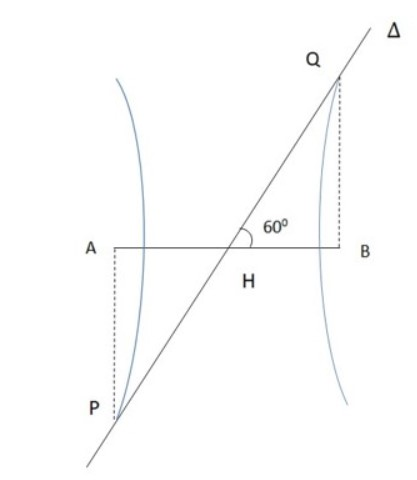
\includegraphics[scale=0.8]{../figs/giaothoasong-h7.jpg}
	\end{center}
	
	Ta có:
	
	$$\text{PA}=\text{QB}=\text{HB}\tan {{60}^\circ}=10\sqrt{3}\,\text{cm}.$$
	
	$$\text{PB}=\text{QA}=\sqrt{A{{B}^{2}}+P{{A}^{2}}}=10\sqrt{7}\,\text{cm}.$$
	
	Bước sóng là
	$$\lambda =\dfrac{v}{f}=3\,\text{cm}.$$
	
	Vì hai nguồn cùng pha nên:
	
	$$\Delta {{d}_\text{P}}\le k\lambda \le \Delta {{d}_\text{Q}}$$		
	$$\Rightarrow \text{PA}-\text{PB}\le k\lambda \le \text{QA}-\text{QB}$$		
	$$\Rightarrow 10\sqrt{3}-10\sqrt{7}\le 3k\le 10\sqrt{7}-10\sqrt{3}$$		
	$$\Rightarrow \dfrac{10\sqrt{3}-10\sqrt{7}}{3}\le k\le \dfrac{10\sqrt{7}-10\sqrt{3}}{3}$$		
	$$\Rightarrow -3,05\le k\le 3,05$$		
	$$\Rightarrow k\in \left\{ 0;\pm 1;\pm 2;\pm 3 \right\}$$
	
	Vậy có 7 điểm dao động với biên độ cực đại.
}
%%%%%%%%%%%Câu 10%%%%%%%%%%%%%%
\item \mkstar{4}

\cauhoi{
	
	Tại mặt chất lỏng, hai nguồn $\text{S}_1$, $\text{S}_2$ cách nhau $13\,\text{cm}$ dao động theo phương thẳng đứng với phương trình $u_1=u_2=A\cos 40\pi t\ \text{cm}$ ($t$ tính bằng s). Tốc độ truyền sóng trên mặt chất lỏng là $80\,\textrm{cm/s}$. Ở mặt chất lỏng, gọi $\Delta$ là đường trung trực của S$_1$S$_2$. M là một điểm không nằm trên $\text{S}_1\text{S}_2$ và không thuộc $\Delta$, sao cho phần tử chất lỏng tại M dao động với biên độ cực đại và cùng pha với hai nguồn. Khoảng cách ngắn nhất từ M đến $\Delta$ là
	\begin{mcq}(4)
		\item $\text{2,00}\,\text{cm}$.
		\item $\text{2,46}\,\text{cm}$.
		\item $\text{3,07}\,\text{cm}$.
		\item $\text{4,92}\,\text{cm}$.
	\end{mcq}
	
}

\loigiai{
	\textbf{Đáp án C.}
	
	\begin{center}
		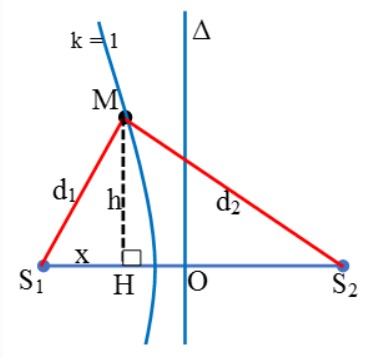
\includegraphics[scale=0.8]{../figs/giaothoasong-h8.jpg}
	\end{center}
	
	Điều kiện để M dao động cực đại và đồng pha với hai nguồn là
	$$\begin{cases}
		d_2-d_1=k\lambda\\
		d_1+d_2=n\lambda.
	\end{cases}$$
	với $n$, $k$ cùng chẵn hoặc cùng lẻ.
	
	Để M gần $\Delta$ nhất thì $k = 1$ và $n$ khi đó có thể nhận các giá trị lẻ 1, 3…..thỏa mãn bất đẳng thức tam giác
	$$d_1+d_2>\text{S}_1\text{S}_2=13\Rightarrow n>\dfrac{13}{\lambda}\Rightarrow n>\text{3,25}.$$
	
	Vậy $n_\text{min}=5$ (do $n$ lẻ).
	
	Ta có:
	$$\begin{cases}
		d_2-d_1=4\\
		d_1+d_2=20
	\end{cases}
	\Rightarrow
	\begin{cases}
		d_2=12\,\text{cm}\\
		d_1=8\,\text{cm}.
	\end{cases}$$
	
	Từ hình vẽ:
	$$\begin{cases}
		d_1^2=8^2=x^2+h^2\\
		d_2^2=12^2=(13-x)^2+h^2
	\end{cases}
	\Rightarrow x=\text{3,42}\,\text{cm}.$$
	
	Vậy khoảng cách giữa M và $\Delta$ khi đó bằng
	$$\text{HO}=\text{OS}_1-\text{S}_1\text{H}=\dfrac{13}{2}-\text{3,42}=\text{3,07}\,\text{cm}.$$
}
	
\end{enumerate}
\loigiai{\textbf{Đáp án}
	\begin{center}
		\begin{tabular}{|m{2.8em}|m{2.8em}|m{2.8em}|m{2.8em}|m{2.8em}|m{2.8em}|m{2.8em}|m{2.8em}|m{2.8em}|m{2.8em}|}
			\hline
			1. C & 2. B & 3. C & 4. D & 5. C & 6. C  & 7. B  & 8. B & 9. D & 10. A\\
			\hline
			11. B & 12. B & 13. A & 14. C & 15. B & 16. A  & 17. C  & 18. C & 19. B & 20. D\\
			\hline
			21. C & 22. B & 23. B & 24. C & 25. B & 26. D  & 27. C  & 28. A & 29. A & 30. C\\
			\hline
		\end{tabular}
\end{center}}